\documentclass[a4paper,12pt]{article}

% Packages
\usepackage{graphicx}  
\usepackage{geometry}  
\usepackage{hyperref}  
\usepackage{titlesec}  
\usepackage{enumitem}  
\usepackage{tikz}
\usetikzlibrary{positioning}

% Page setup
\geometry{left=2.5cm, right=2.5cm, top=2.5cm, bottom=2.5cm}

% Title Formatting
\titleformat{\section}{\Large\bfseries}{\thesection}{1em}{}

\begin{document}

% Title
\begin{center}
    {\LARGE \textbf{HCLI - Habit Tracker CLI}}\\[0.5cm]
    {\Large \textbf{Conception Phase}}\\[0.3cm]
    {\small Author: Alejandro Moral Aranda \hspace{1cm} Date: \today}
    \hrule
\end{center}

\section{Concept Overview}
HCLI is a lightweight, CLI-based habit tracker that allows users to efficiently manage and analyze habits without distractions. It provides commands to add, track, and review habits, storing data in JSON for easy access.

\section{Approach}
Users interact with HCLI using simple commands:
\begin{itemize}
    \item \texttt{python main.py add "Workout" daily} - Adds a habit.
    \item \texttt{python main.py check "Workout"} - Logs completion.
    \item \texttt{python main.py summary} - Shows progress.
\end{itemize}
Built with Python, Typer, and Rich, the system ensures a seamless user experience.


\section{System Architecture}
HCLI consists of:
\begin{itemize}
    \item \textbf{CLI Interface} - Processes user commands.
    \item \textbf{Data Manager} - Stores and retrieves habits.
    \item \textbf{Analytics Engine} - Tracks habit streaks and reminders.
\end{itemize}
The development of HCLI follows a structured approach: implementing core CLI commands, managing data storage, enhancing user interaction, providing analytics and visualization, enabling configuration, and ensuring reliability through testing.



% UML Diagram
\begin{center}
 \title{UML Class Diagram for HCLI}
   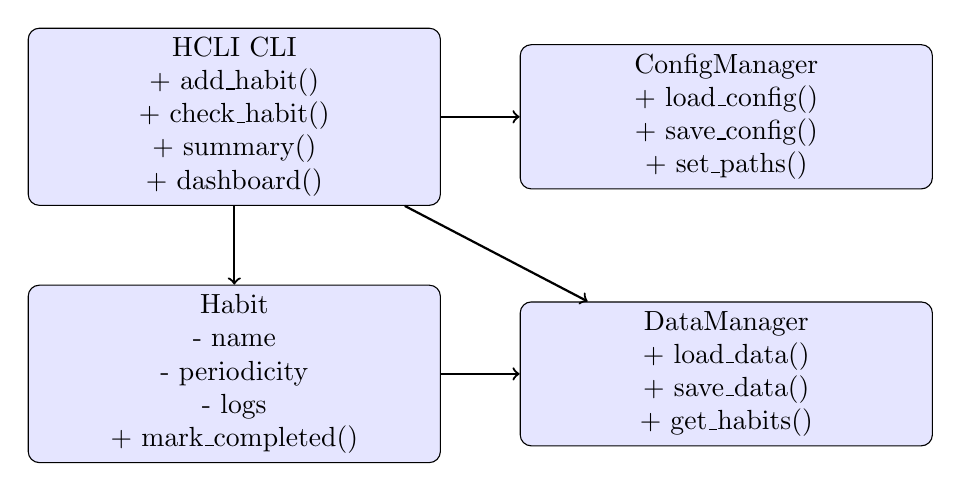
\begin{tikzpicture}[
        class/.style={rectangle, draw, fill=blue!10, rounded corners, text width=5cm, minimum height=1.5cm, align=center},
        interface/.style={rectangle, draw, fill=red!10, dashed, text width=5cm, minimum height=1.5cm, align=center},
        arrow/.style={->, thick}
    ]

    % Classes
    \node[class] (cli) {HCLI CLI \\ + add\_habit() \\ + check\_habit() \\ + summary() \\ + dashboard()};
    \node[class, below=of cli] (habit) {Habit \\ - name \\ - periodicity \\ - logs \\ + mark\_completed()};
    \node[class, right=of habit] (data) {DataManager \\ + load\_data() \\ + save\_data() \\ + get\_habits()};
    \node[class, right=of cli] (config) {ConfigManager \\ + load\_config() \\ + save\_config() \\ + set\_paths()};

    % Relationships
    \draw[arrow] (cli) -- (habit);
    \draw[arrow] (cli) -- (data);
    \draw[arrow] (cli) -- (config);
    \draw[arrow] (habit) -- (data);
 
    \end{tikzpicture}
    
\end{center}



\end{document}
